\documentclass[12pt]{article}
\usepackage{graphicx}
\usepackage{color}
\usepackage{xspace}
\usepackage{listings}
\definecolor{webgreen}{rgb}{0,0.5,0}
\definecolor{purple}{rgb}{0.8,0.2,0.7}

\lstset{language=C++,commentstyle=\color{red},identifierstyle=,keywordstyle=\color{webgreen},stringstyle=\color{purple},basicstyle=\color{blue}\scriptsize\tt,escapechar=\@,xleftmargin=5mm,aboveskip=5pt,belowskip=0pt,lineskip=-1pt,showstringspaces=false}
\lstset{language=Python}

\newcommand{\CPP}{C\texttt{++}\xspace}  % C++

\begin{document}
\title{Fe55 analysis using ``RV''}
\author{Robert Lupton}
\maketitle

\section{Introduction}

Andy Rasmussen kindly provided me with some legacy C used to analyse Fe55 data,
\texttt{medpict\_lsst.c}, \texttt{rv\_ev2pcf.c}, \texttt{rv\_ev2xygpx.c}, and \texttt{rv\_gflt.c}. These
are designed to be used in a unix pipeline, \textit{e.g.}
\begin{lstlisting}
medpict_lsst -b -f c -c -e < fe55_files*.fits > evlist.dat
cat evlist.dat | rv_gflt 30 10 -g 0 2 3 4 6 | rv_ev2xygpx 30 10 p9
\end{lstlisting}

In order to explore the use of the LSST DM stack while testing and manufacturing the LSST camera,
I took a look at these C codes with the intention of:
\begin{itemize}
  \item Seeing to what extent the code is production quality\footnote{\textit{N.b.} Andy R. made
    no representation that the code should be used in production;  rather it is part of his personal toolset}
  \item Discovering how hard it would be to rewrite the code in \CPP
  \item Finding how much of the functionality is already present in the DM stack
  \item Exploring how easily the DM stack can be used, in conjunction with this code, to analyse Fe55 data
\end{itemize}

\section{Analysis of Existing Code}

The code shows its age;  it was originally written for a pre-C89 compiler (\textit{e.g.} no
prototypes; old style function declarations) and has been only partially updated.
The compilers\footnote{I used both gcc and clang} generated many warnings, and some of them turned out to
be real bugs (\textit{e.g.} adding function prototypes uncovered mistakes in
arguments being passed to functions; it's unclear why the code didn't crash outright in some cases).
Fixing these issues allowed the code to be compiled with a \CPP compiler.

Some of the code has been written in style that is difficult to read, ostensibly to
make it run faster (\textit{e.g.} the lookup tables designed to handle bias
subtraction). This is particularly true of the \texttt{medpict} program used to
detect Fe55 events. However, general software engineering experience has shown that it's
preferrable to sacrifice a few percent of performance in favor of code clarity. Clear code
leads to faster development, easier maintenence, and less bugs. Human time
spent on detecting and fixing bugs is typically significantly more expensive than any 
realized savings due to highly optimized code, and with modern compilers we're often not
required to actually make the sacrifice. 

There is a lot of code repetition between the various routines, quite a lot of hard-coded numbers, and
extensive use of global variables, reducing the code's reusability.

The example pipeline I gave above used a temporary file rather than a pure pipline; this is in fact necessary
due to the assumptions that the code makes about the POSIX \texttt{read} call always returning as many bytes
as are requested.

The code as written mixes up the classification of the events with the generation of the histograms, and
generates the outputs in a format designed to be used
with \texttt{QDP}, a slightly unusual front-end to \texttt{pgplot}.

All of the identified issues are understandable in light of the organic
evolution and intent behind this code, its age, and the lack of a standard
``toolbox'' of image processing routines that one could rely on.  Below, I
show how this code could be written today, using LSST DM stack routines for
common tasks.

\section{An experimental rewrite in \CPP}

\begin{figure}
\begin{lstlisting}
def processImage(thresh, fileName, grades=range(8), searchThresh=None, split=None,
                 calcType=ras.HistogramTable.P_9,
                 outputHistFile=None, outputEventsFile=None):

    if searchThresh is None:
        searchThresh = thresh

    ccd, image = cameraGeom.assembleCcd(fileName, trim=True)
    # Run detection
    fs = afwDetect.FootprintSet(image, afwDetect.Threshold(searchThresh))

    # Convert all the peaks within the detections to Events
    for foot in fs.getFootprints():
        for i, peak in enumerate(foot.getPeaks()):
            peakPos = afwGeom.PointI(peak.getIx(), peak.getIy())
            amp = ccd.findAmp(peakPos, True)
                
            events.append(ras.Event(image, peakPos, frameNum, amp.getId().getSerial()))
    #
    # Prepare to go through all our events, building our histograms
    #
    if split is None:
        split = int(0.33*thresh)

    filt = sum([1 << g for g in grades])

    table = ras.HistogramTable(thresh, split)
    table.setFilter(filt)
    table.setCalctype(calcType)
    table.setReset(ras.HistogramTable.T1, 0.0)

    # Process the events
    status = [table.process_event(ev) for ev in events]

    # Output
    with open(outputEventsFile, "w") as fd:
        for stat, ev in zip(status, events):
            if stat:
                print >> fd, "%d %d %d %d %g %d" % (ev.x, ev.y, ev.grade, ev.sum, ev[4], ev.p9)

    with open(outputHistFile, "w") as fd:
        table.dump_head(fd, "unknown", sum(status))
        table.dump_hist(fd)
    #table.dump_table()
\end{lstlisting}
\caption{A minimalistic processing script for Fe55 events}
\label{processImage}
\end{figure}

\begin{figure}
\lstset{language=Python}
\begin{lstlisting}
def plot_hist(table):
    fig = plt.figure()
    axes = fig.add_axes((0.1, 0.1, 0.85, 0.80))

    x = np.arange(0, table.MAXADU)
    for g, label in enumerate(["N(S)",  "N(S+)", "N(Pv)",  "N(Pl)",
                               "N(Pr)", "N(P+)", "N(L+Q)", "N(O)",]):
        axes.step(x, table.histo[g], label="%d %s" % (g, label), where='mid')

    axes.set_xlabel("Pulse Height (ADU)")
    axes.set_ylabel("lg(N)")
    axes.set_xlim(table.min_adu - 10, table.max_adu + 10)

    axes.legend(loc=1)
    fig.show()
\end{lstlisting}
\caption{A minimalistic plotting script}
\label{plot_hist}
\end{figure}

\begin{figure}
  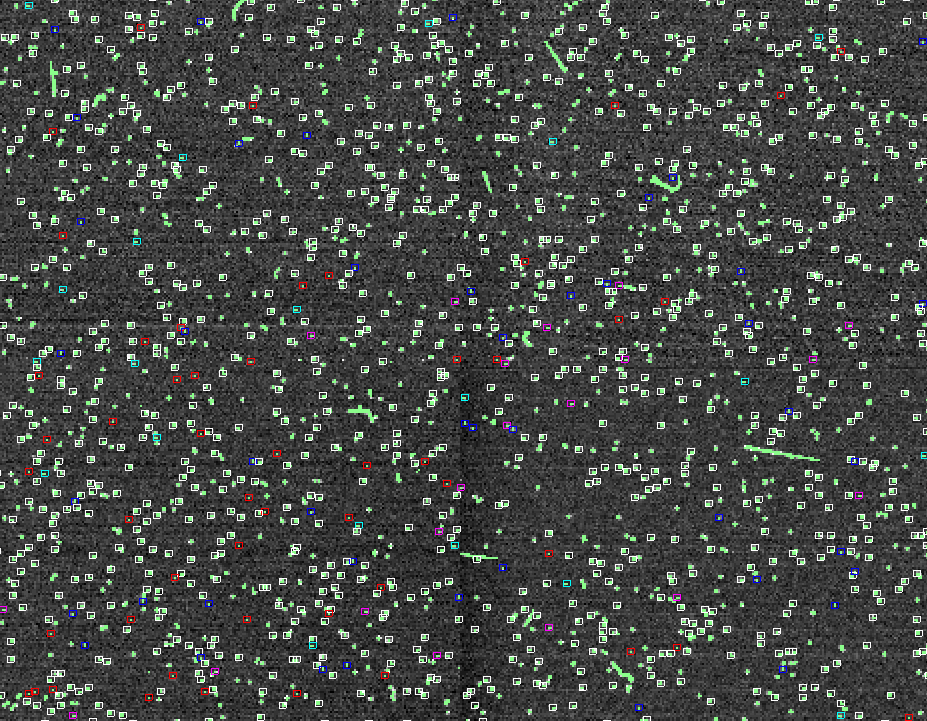
\includegraphics[width=\the\hsize]{fe55-ds9}
  \caption{The central part of the CCD (the corners of amps 4, 5, 12, and 13) showing Fe55 events
    and cosmic ray hits.  Detected
    pixels are a tasteful light green, and the desired grades of event (0 2 3 4 6) are coloured
    as in the caption for Fig. \ref{eventsHistogramGain} (with black replaced by white).  The
    bias was estimated separately for each row of each amp due to significant (and correlated)
    spatial structure in amps 9, 11, 13, and 15.
  }
  \label{ds9Events}
\end{figure}

\begin{figure}
  \hspace*{-10mm}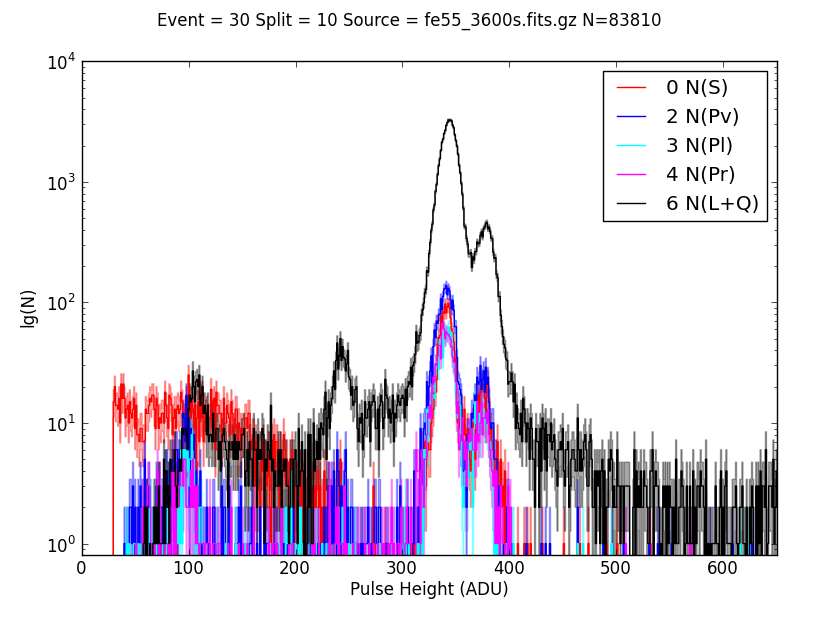
\includegraphics[height=12cm]{fe55-gain}
  \caption{A histogram of events.  Each amplifier has been corrected for its gain in
    such a way that the individual histograms line up
  }
  \label{eventsHistogramGain}.
\end{figure}

\begin{figure}
  \hspace*{-10mm}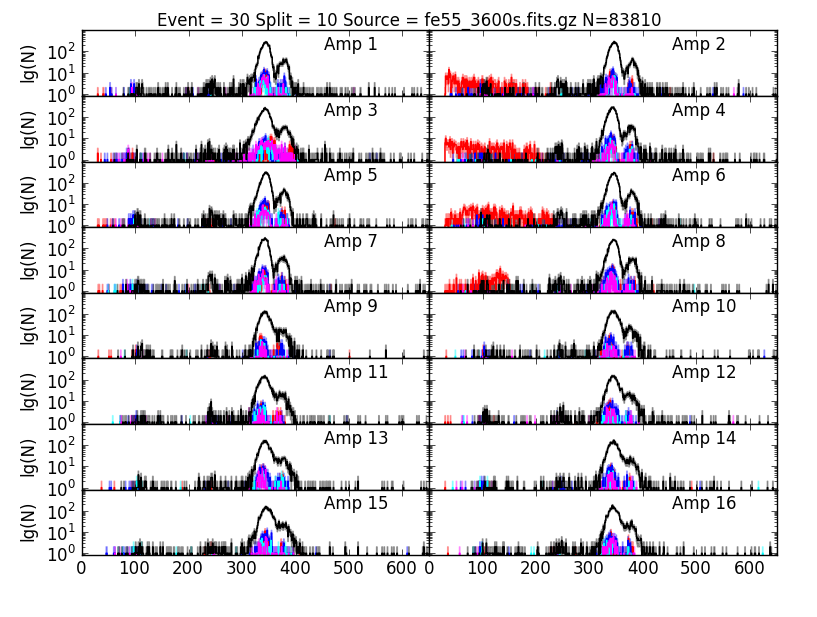
\includegraphics[height=12cm]{fe55-gain-perAmp}
  \caption{A histogram of events for each amplifier.  Each amplifier has been corrected for its gain in
    such a way that the individual histograms line up
  }
  \label{eventsHistogramPerAmp}
\end{figure}

I checked Andy's code into git at \texttt{git\@git.lsstcorp.org:contrib/fe55}, and proceeded
with a rewrite into \CPP.

While working on refactoring the code I checked that I got the exact results that the initial C code had
produced (these regression tests are run as part of the regular build).  This required me to emulate various
features of the C code (\textit{e.g.} its definition of a peak); a number of
these may actually be bugs.

When the prototype-related issues were fixed I was able to compile Andy's C with a \CPP compiler, but I decided
that rather than make a minimal translation I'd re-write the algorithms into rather more idiomatic code;
I did not change the basic approach of statically initialised tables.  I'd
capture all the globals in a \texttt{HistogramTable} class, and handle as much of possible as the
classification via an \texttt{Event} class.  I bound the \CPP to python using swig, and mapped the histograms
to \texttt{numpy} using Jim Bosch's \texttt{ndarray} class, permitting the use of python's \texttt{matplotlib}
(the DM standard plotting library); see Figs. \ref{processImage} and \ref{plot_hist}.  Visualisation of images
and events was done via the DM's \texttt{ds9} interface.

I was able to entirely replace the C codes with python calling DM's \CPP primitives, \textit{e.g.}
object detection (a large portion of \texttt{medpict}) is simply:
\begin{lstlisting}
  fs = afwDetect.FootprintSet(image, afwDetect.Threshold(searchThresh))
\end{lstlisting}
I could write all three \texttt{rv\_*.c} routines as simple routines manipulating \texttt{HistogramTables}.
For example, the shell command
\begin{verbatim}
fe55 fe55_3600s.fits.gz --grades 0 2 3 4 6 --calc P_9 --thresh 30 \
     --split 10 --plot --plotByAmp --assemble --ds9
\end{verbatim}
calls a slightly more complicated version of the routine shown in Fig. \ref{processImage} to
display the selected grades of event on \texttt{ds9} (see Fig. \ref{ds9Events}) and generate
the histogram in Fig. \ref{eventsHistogramPerAmp} (omitting \texttt{--plotByAmp} generates
Fig. \ref{eventsHistogramPerAmp}).  All this functionality is, of course, also available
interactively from the python prompt.
These per-amp plots were possible because of the replacement of global tables by the \texttt{HistogramTable}
objects.  \textit{N.b.} These histogram were corrected for the per-amplifier gain by estimating the position
of the peak of each separate histogram.

We see that the grade 0 (single pixel events) are concentrated in amps 2, 4, 6, and 8; part of
amp 4 may be seen in the south west quadrant of Fig. \ref{ds9Events}.

\subsection{\texttt{cameraGeom}; a description of the data layout}

The LSST DM stack supports a description of the way that amplifiers fit into CCDs, as well as how the CCDs are
fitted into rafts, and the rafts into the camera; ``\texttt{lsst::afw::cameraGeom}''.
In order to process Fe55 data we only need the first part
of this (amps fitting into CCDs), and we don't need the soon-to-be-replaced on-disk description of
the \texttt{cameraGeom}.  An alternative is to use the header keywords that describe the mapping
from amp to CCD coordinates (\texttt{LTV1} \textit{etc.}).

The advantage of the DM approach is that it encapsulates the data in classes with useful methods,
\textit{e.g.} given a \texttt{cameraGeom::Ccd ccd} I can ask \texttt{ccd.findAmp(afwGeom::PointI(x, y))}
to find to which amplifier a pixel \texttt{x, y} belongs.

I wrote some code to parse the headers (a DM \texttt{PropertyList}) to construct the \texttt{cameraGeom}
objects, but unfortunately:
\begin{itemize}
  \item The headers were not complete (\texttt{e.g.} no definition of the bias pixels)
  \item The headers appeared to be incorrect (see Appendix \ref{badHeader})
  \item The headers don't include \textit{e.g.} the amplifier's gain.
\end{itemize}

Putting these configuration parameters into an external file allows us to work with data with incorrect
headers, and also allows us to version things like the gain and readnoise.  It is, of course, possible
to validate the externally specified data from the headers.

In Fig. \ref{processImage},
\begin{lstlisting}
    ccd, image = cameraGeom.assembleCcd(fileName, trim=True)
\end{lstlisting}
uses a light-weight \texttt{cameraGeom} specification to read all 16 amplifiers, correct for bias
and gain, trim the overclock, and assemble a \texttt{4096x4000} CCD image.

\appendix
\section{Problems in the Fe55 Data Headers}
\label{badHeader}

I'm not an expert on the IRAF mosaic geometry headers, but I think the geometry
as stored in the headers is incorrect --- I'd be happy to be proved wrong.

For example, channel 1's header has:
\begin{verbatim}
DATASEC = [1:542,1:2022]
DETSEC  = [0:542,0:2022]
DETSIZE = [0:4336,0:4044]
\end{verbatim}
(so \texttt{DETSEC} is  543x2023 and \texttt{DETSIZE} is 4337x4045)
If the 0 is correct, it implies that there's logically 1 pre-scan pixel so \texttt{Cx} starts at 0.0

When we look at channel 16 we see
\begin{verbatim}
LTV1 =  542
LTV2 = 4044
\end{verbatim}
which means that the pixel with \texttt{(Ic, Il) == (542, 4044)} maps to \texttt{(Cx, Cy) = (0.0, 0.0)}

The problems with this theory are:
\begin{enumerate}
\item There are more than 1 overscan pixels (I think 10)
\item The size of the DETSEC and DETSIZE are wrong --- they should be e.g. [0:541, 0:2021]
\end{enumerate}

I think that a more likely explanation is that there's an off-by-one error in \texttt{LTV[12]} for the 8
rotated channels at the top of the chip; all the problems are resolved by incrementing their \texttt{LTV[12]}
by 1.

\end{document}
